\smallframetitle

\section{From 08/07/24 to 12/07/24}
\insertsectionframe

\subsection{further advancement on road detection}
\insertsubsectionframe

\begin{frame}{Little advancement}
    \begin{block}{City name detection}
        For each city detected, we find the closest base station to the center of the said city. 
        We then declare that the name of the city is the value contained in the field "nom\_com" of the base station.
    \end{block}

    \begin{figure}
        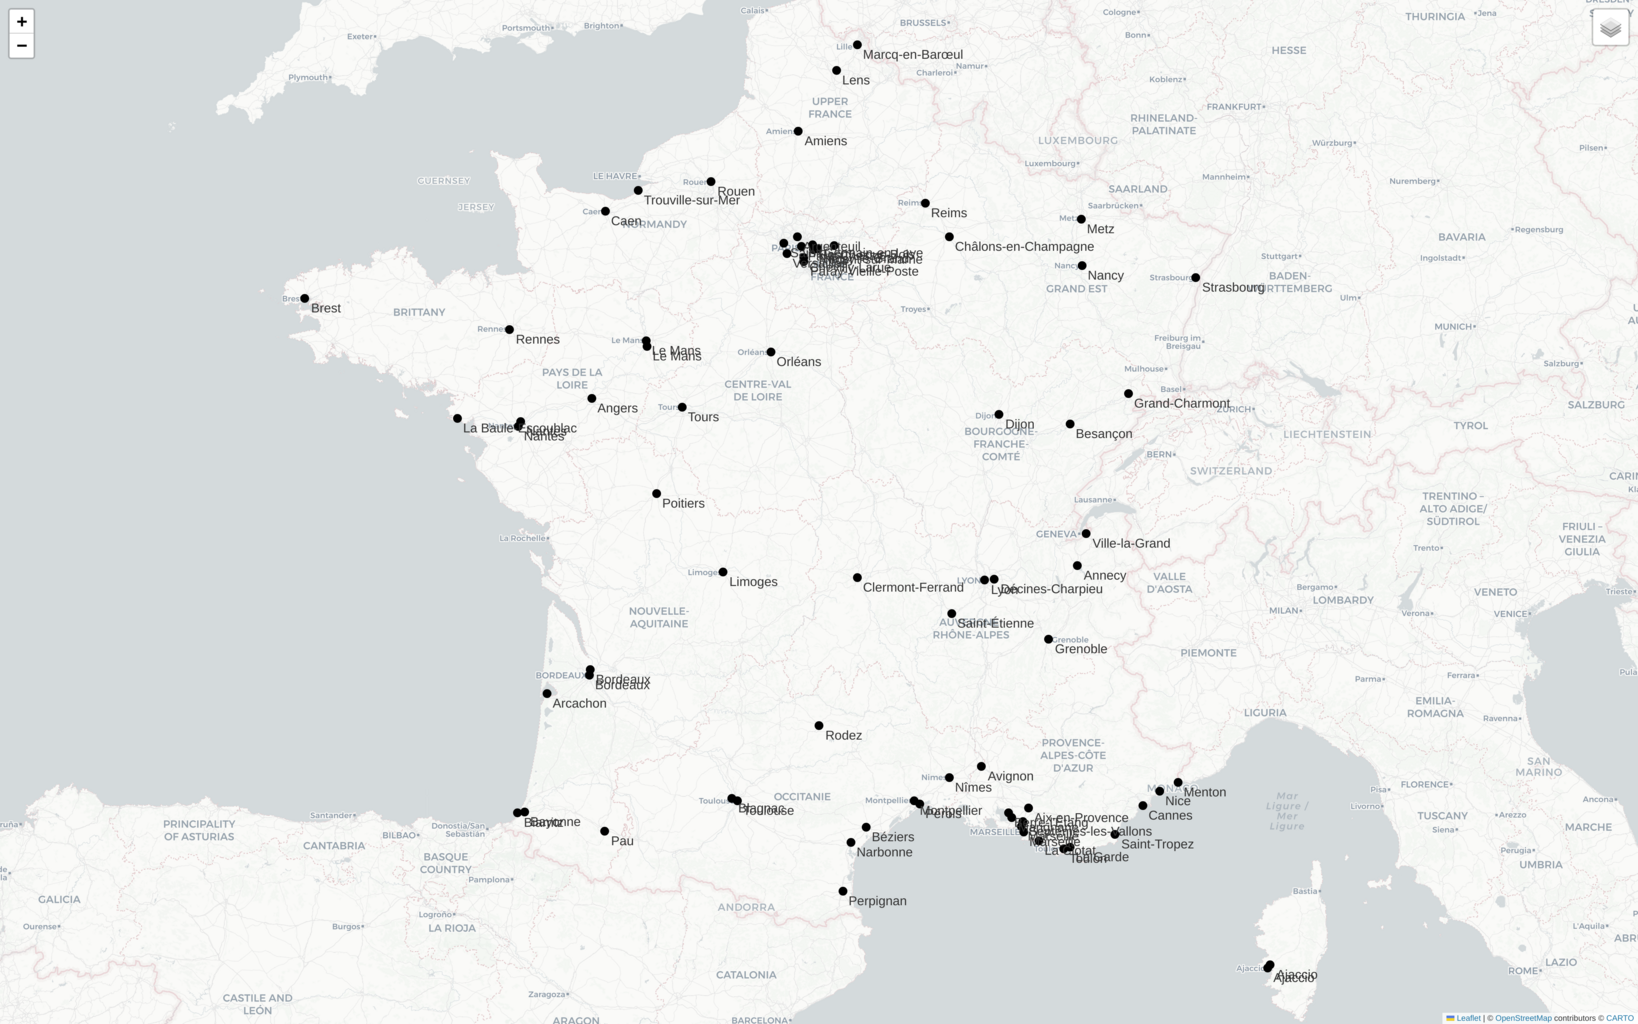
\includegraphics[height=0.4\paperheight]{images/road_detection/cities_centers_with_name.png}
        \caption{Cities centers with name}
    \end{figure}
\end{frame}

\begin{frame}{New method (1/2)}
    \begin{block}{Edges weight}
        For each couple of cities, we compute a weight using this formula :
        $$w_{\text{city1, city2}} = \frac{\min(\text{size(city1)},\text{size(city2)})}{\text{dist(city1, city2)}}$$
        With the size of a city refering to the number of base stations detected inside that city.
        
        We the keep all the edges whose weight is superior to a certain value.
    \end{block}

    \begin{figure}
        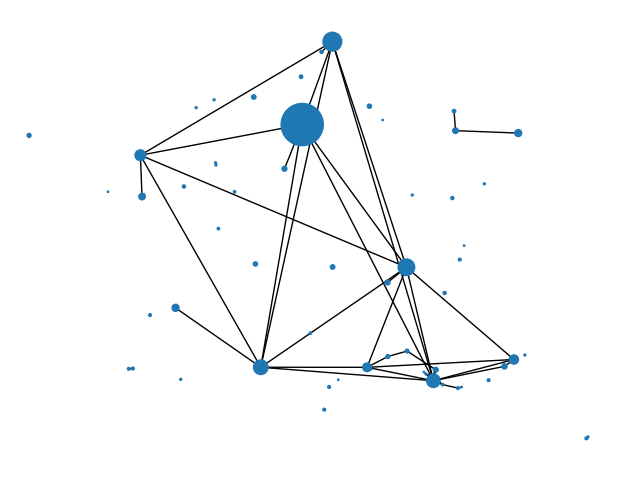
\includegraphics[height=0.3\paperheight]{images/road_detection/edges_weight_filtration.png}
        \caption{weight filtration, cap value = $0.1$}
    \end{figure}
\end{frame} 

\begin{frame}{New method (2/2)}
    \begin{block}{Edges weight}
        We then apply the angle criterion to the resulting graph
    \end{block}

    \begin{figure}
        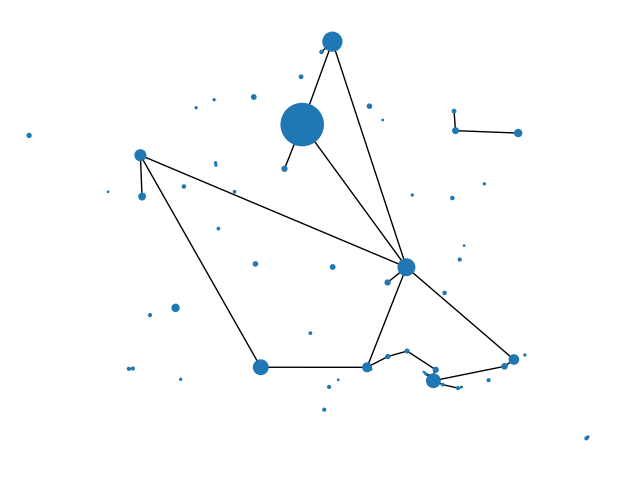
\includegraphics[height=0.4\paperheight]{images/road_detection/edges_weight_angle_filtration.png}
        \caption{weight and angle filtration, cap value = $0.1$, angle value = $15$ degrees}
    \end{figure}
\end{frame} 

\subsection{Method for Finding Neighboring Base Stations Using Voronoi Diagrams}
\insertsubsectionframe

\begin{frame}{Voronoi Diagrams for Neighboring Base Stations}
    \begin{itemize}
        \item The method uses Voronoi diagrams to determine the neighborhood of base stations.
        \item If the cells share a common boundary, the base stations are considered neighbors.
    \end{itemize}
    \begin{figure}
        \centering
        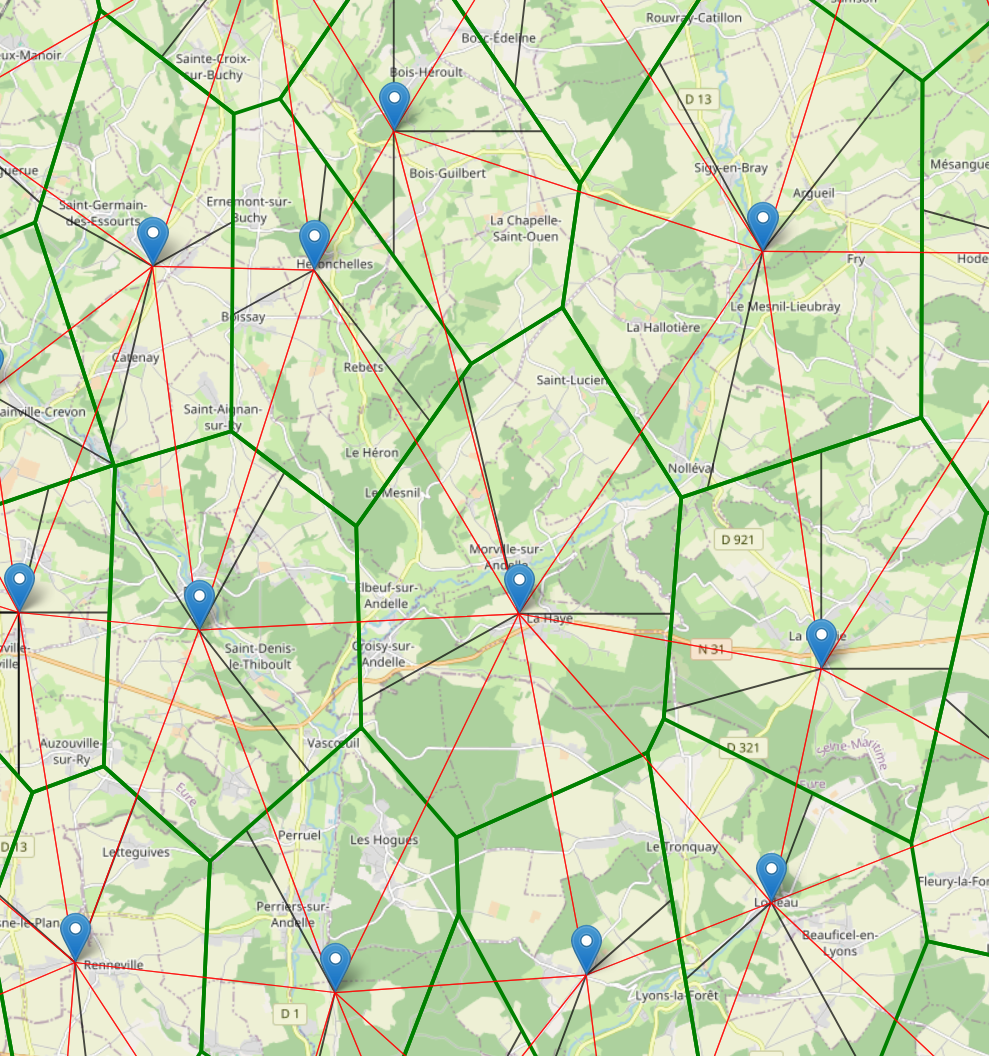
\includegraphics[width=0.3\textwidth]{images/Altair/voron-neighb.png} 
        \caption{Voronoi Diagram Showing Neighboring Base Stations}
    \end{figure}
\end{frame}

\begin{frame}{Analysis of Results}
    \begin{block}{Explanation of inaccuracy}
        \begin{itemize}
            \item The method considers only geometric proximity without accounting for actual network topology or physical barriers.
            \item It's analogous to using Delaunay triangulation and assuming all neighboring stations in the triangulation are true neighbors.
        \end{itemize}
    \end{block}
    \begin{columns}
        \begin{column}{0.5\paperwidth}
            \begin{figure}
                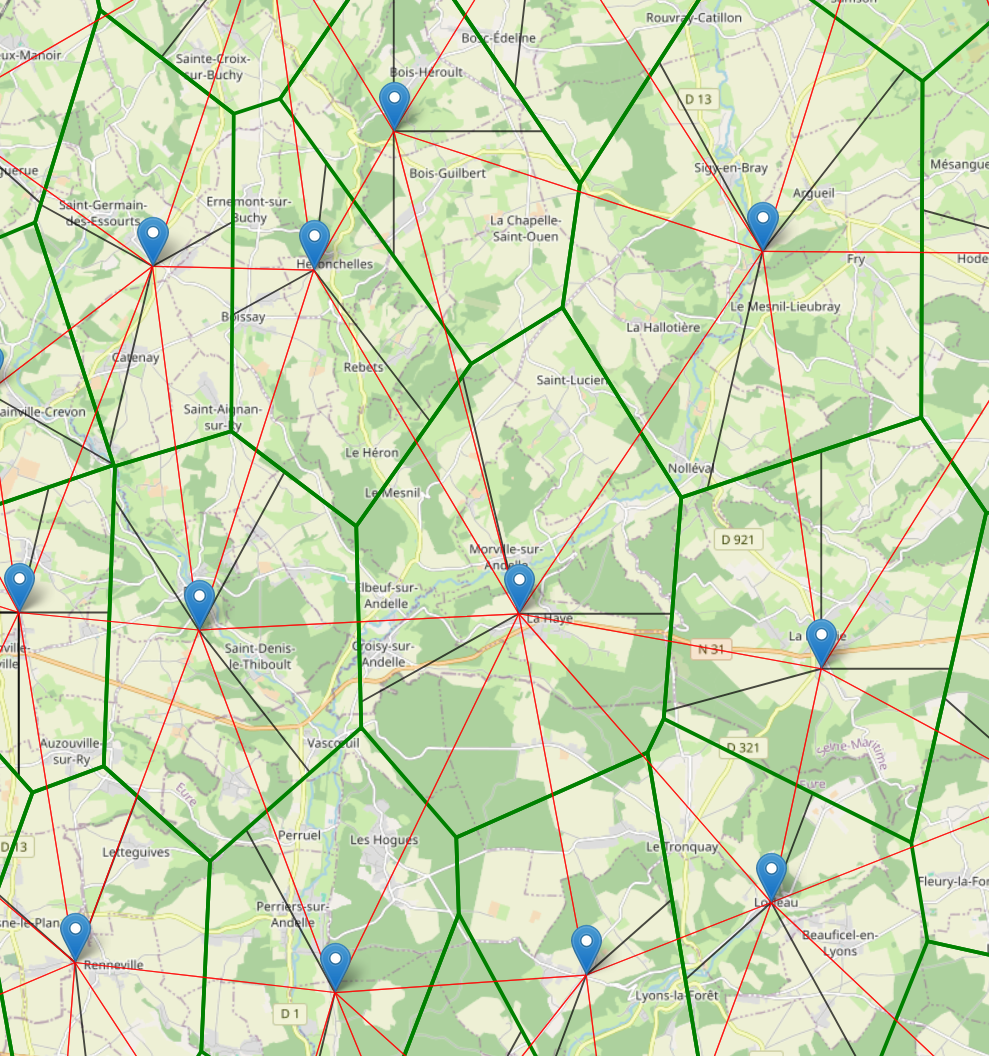
\includegraphics[height=0.3\paperheight]{images/Altair/voron-neighb.png}
                \caption{Voronoi Diagram Showing Neighboring Base Stations}
            \end{figure}
        \end{column}
        
        \begin{column}{0.5\paperwidth}
            \begin{figure}
                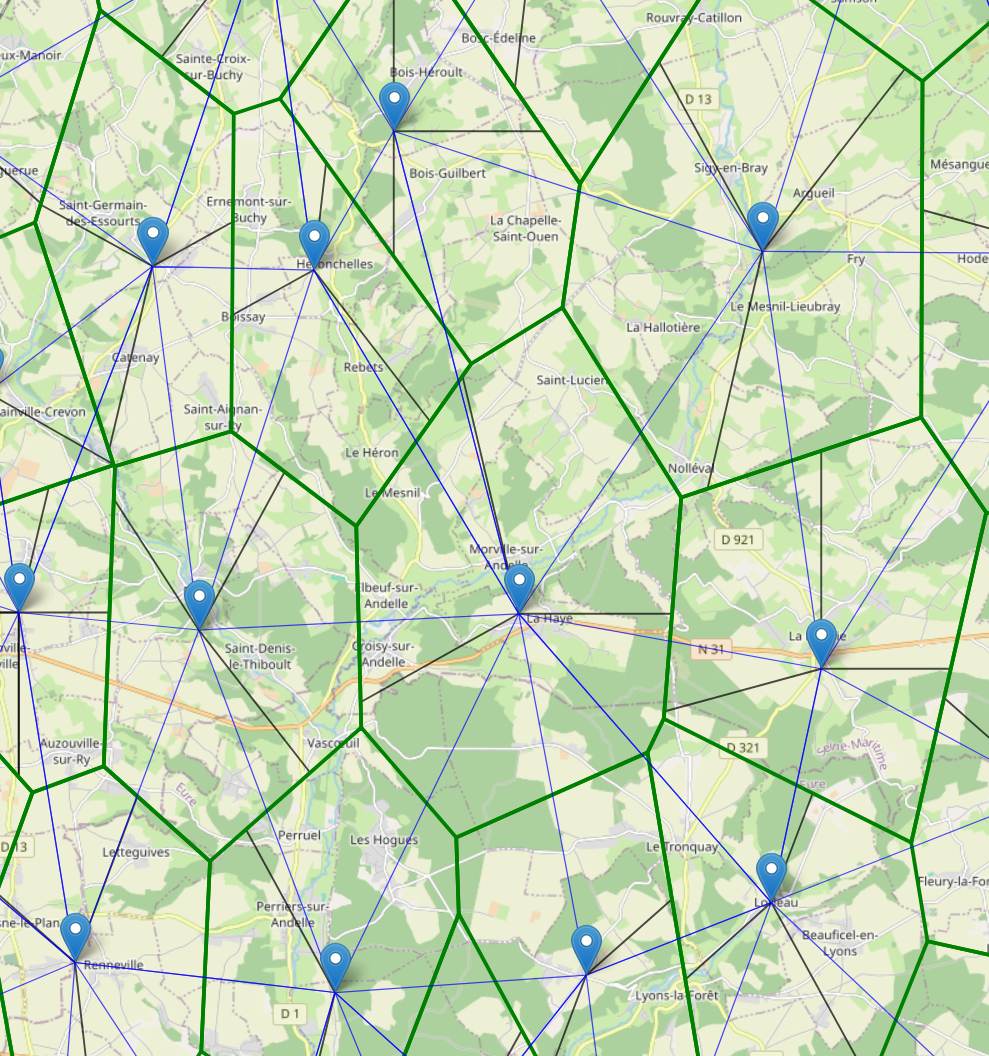
\includegraphics[height=0.3\paperheight]{images/Altair/delon-neighb.png}
                \caption{Delaunay Triangulation of Base Stations}
            \end{figure}
        \end{column}
    \end{columns}
\end{frame}


\subsection{Introduction to the New Method for Determining Neighboring Base Stations}
\insertsubsectionframe

\begin{frame}
    \frametitle{New Method for Determining Neighboring Base Stations}
    \begin{itemize}
        \item The method uses Delaunay triangulation to identify potential neighboring base stations.
        \item Verification of neighboring status is done by checking antenna coverage angles.
        \item Stations are considered neighbors if their antenna directions align within their coverage angles.
    \end{itemize}
    \begin{block}{Determining Antenna Coverage Angles}
        \begin{itemize}
            \item Calculate the coverage angle for each antenna by dividing 360 degrees by the number of unique azimuths.
            \item This gives the angular sector covered by each antenna on the station.
        \end{itemize}
    \end{block}
    \end{frame}


\begin{frame}
    \frametitle{Validating Neighboring Status}
    \begin{itemize}
        \item For each pair of stations connected by an edge, check the direction of the connecting line.
        \item Compare this direction with the antenna coverage angles of both stations.
        \item If the direction falls within the coverage angles, the stations are real neighbors.
    \end{itemize}
    \begin{figure}
        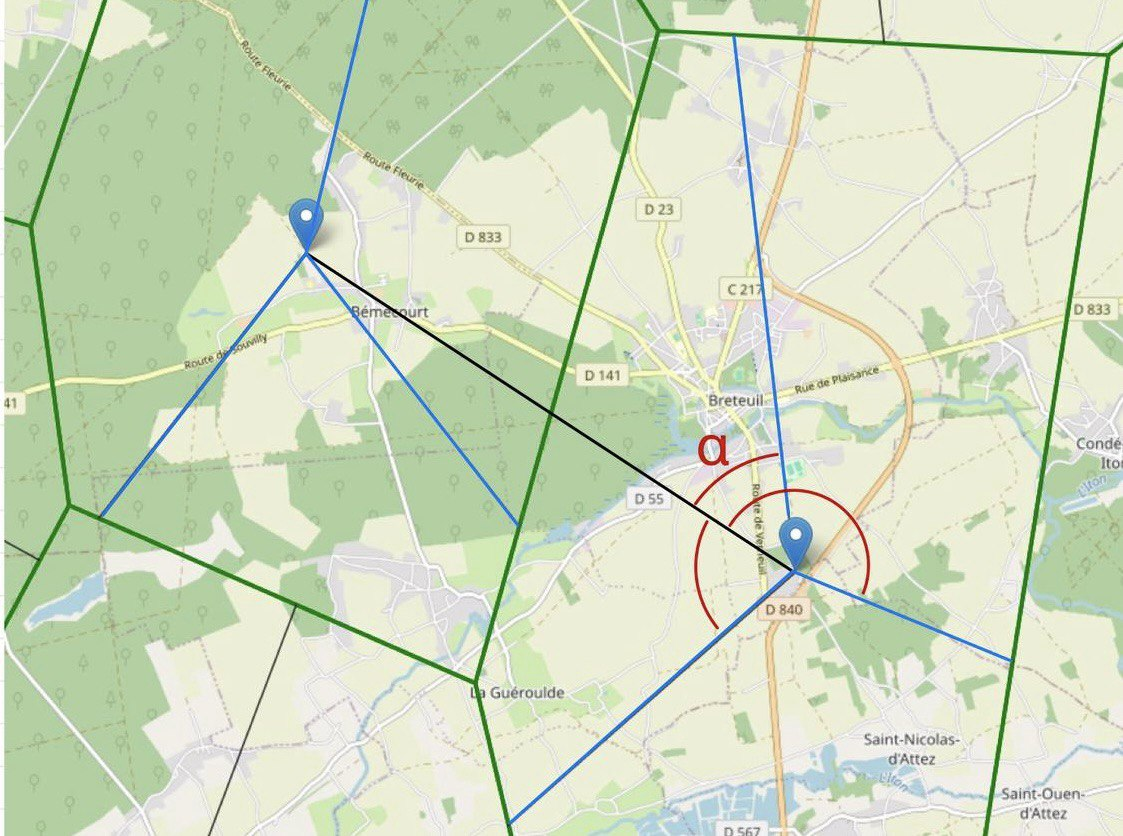
\includegraphics[height=0.5\paperheight]{images/Altair/antenn-angle.png} 
        \caption{Validation of Neighboring Status}
    \end{figure}
\end{frame}
    

\begin{frame}
    \frametitle{Detailed Steps with Formulas}
    \begin{itemize}
        \item Calculate Direction of the Connecting Line:
        \[ \theta = \arctan2(y_2 - y_1, x_2 - x_1) \]
        where \((x_1, y_1)\) and \((x_2, y_2)\) are the coordinates of the two base stations.
        
        \item Calculate the Antenna Coverage Angles:
        \begin{align*}
        \text{Coverage Start Angle} &= A - \frac{B}{2} \\
        \text{Coverage End Angle} &= A + \frac{B}{2}
        \end{align*}
        For an antenna with azimuth \(A\) and beamwidth \(B\).

        \item Validate if the Connecting Line Falls Within Coverage Angles:
        Normalize angles to be within \([0^\circ, 360^\circ]\).
        Check if the direction \(\theta\) falls within \([A - \frac{B}{2}, A + \frac{B}{2}]\).

        \item Bi-Directional Check:
        Repeat the validation from both base stations' perspectives.
        If \(\Delta \theta\) for both stations is within the beamwidth, they are considered true neighbors.
    \end{itemize}
\end{frame}


\begin{frame}
    \frametitle{Updating the Dataset}
    \begin{itemize}
        \item Add validated neighboring stations to the dataset.
        \item Update the data frame with pairs of stations identified as real neighbors.
    \end{itemize}
    \begin{block}{Result}
        \begin{itemize}
            \item Improved accuracy in identifying neighboring base stations.
            \item More reliable data for network and coverage analysis.
        \end{itemize}
    \end{block}
    \begin{block}{Summary and Conclusion}
        \begin{itemize}
            \item The new method combines geometric triangulation with antenna direction validation.
            \item This approach enhances the accuracy of identifying neighboring base stations.
            \item This method can be further refined and applied to past methods as an additional criterion.
        \end{itemize}
    \end{block}
\end{frame}